\documentclass[a4paper, 12pt]{article}
\usepackage{bm}
\usepackage{amssymb}
\usepackage{graphicx}
\usepackage{amsmath}
\usepackage{amsfonts}
\usepackage{float}
\usepackage{wrapfig}
\graphicspath{ {images/} }
\begin{document}
\begin{center} 
{\Huge{\textbf{Solitons}}}\\
\end{center}

\section {What are solitons and solitary waves?}
 The study of classical solution of field theory equations which have some good properties like travelling without dissipation, with uniform velocity, shape preservation even after collision are vaguely called solitons and solitary waves. The wave equation in 1+1 dimesions
  $$ \square \phi = \partial^{\mu}\partial_{\mu}\phi = \left(\frac{1}{c^2}\frac{\partial^2}{\partial t^2} - \frac{\partial^2}{\partial x^2} \right)\phi(x,t)=0$$
  is satisfied by any function of the form $f(x-ct)$ because it is made up of plane waves all having the same wave velocity. The second interesting feature of solutions of wave equation is that they retain their original shapes after collision after a very long time. We observe that even a simple addition of term to a wave equation destroys these properties.However it is possible for some equation where both dispersive and non-linear terms cancel each other's effect and the solution satisfies those properties. \textit{We will restrict ourselves to field equations(for any set of coupled fields $\phi_1(\bm x,t),\phi_2(\bm x,t),...$)where the energy density $\epsilon(\bm x,t)$ is some function of the fields $\phi_i(\bm x,t)$.} The space integral is the conserved total energy functional $\bm E[\phi_i]$. We will use the term \textbf{localised} for those solutions whose energy density $\epsilon(\bm x,t)$ at any finite time is localised in space. That is energy density goes to zero at spatial infinity sufficiently fast to be integrable. The properties are stated in terms of their energy density are as follows: 
 \begin{equation}%%%%%%%%%%1%%%%%%%%%%
 \epsilon(\bm x,t)=\epsilon(\bm x - \bm ut) 
 \end{equation}
\textit{ Localised }non-singular solution of (1) is called a \textbf{solitary wave}.
 \begin{equation}%%%%%%%%%%2%%%%%%%%%%
  \epsilon(\bm x,t) \to \sum_{i=1}^{N} \epsilon_0(\bm x -\bm{a_i} - \bm {u_i}t) \quad \textrm{as t} \to  -\infty
 \end{equation}
 Given this configuration at t$= -\infty$, it will evolve according to the non-linear equation. Suppose this evolution is such that 
  \begin{equation}%%%%%%%%%%3%%%%%%%%%%
  \epsilon(\bm x,t) \to \sum_{i=1}^{N} \epsilon_0(\bm x -\bm{a_i} - \bm {u_i}t + \bm{\delta_i}) \quad \textrm{as t} \to  +\infty
 \end{equation}
 where $\bm{\delta_i}$ are some constant vectors which is included to represent the possibility that there might be a change in direction after the collision. So solitary waves stisying the above condition are called \textbf{solitons}.
 

\section {Solitary waves in two dimensions(1+1d)} 
We have set(choose potential) the minimum energy to be zero. \textit{For being localised $\epsilon(\bm x,t)$ has to go to zero as x$\to \pm \infty$,} this follows from the definition. Let's see this through some simple illustrations : 
\\
 Adding a simple non-linear term to the wave equation gives
\begin{equation}%%%%%%%%%%4%%%%%%%%%%
\left(\frac{1}{c^2}\frac{\partial^2}{\partial t^2} - \frac{\partial^2}{\partial x^2} \right)\phi(x,t) + \phi^3(x,t)=0
\end{equation}
 The energy functional of the above equation is given by
 \begin{equation}%%%%%%%%%%5%%%%%%%%%%
\bm  E[\phi] = \int_{\infty}^{-\infty} dx \bigg[ \frac{1}{2c^2}\bigg(\frac{\partial\phi}{\partial t}\bigg)^2 +\frac{1}{2}\bigg(\frac{\partial\phi}{\partial x}\bigg)^2 +\frac{1}{4}\phi^4 \bigg]
 \end{equation}
  Since $\phi$'s are real scalar fields the energy functional is minimised by $\phi(x,t) = 0$. Localised solutions of this system if any would asymptotically go to $\phi(x,t) = 0$ as x$\to \pm \infty$, at any given t. Similarly for
 \begin{equation}%%%%%%%%%%6%%%%%%%%%%
\frac{1}{c^2}\frac{\partial^2\phi}{\partial t^2} - \frac{\partial^2\phi}{\partial x^2} -\phi + \phi^3=0
\end{equation}
 
 The energy functional of the above equation is given by
 \begin{equation}%%%%%%%%%%7%%%%%%%%%%
\bm  E[\phi] = \int_{\infty}^{-\infty} dx \bigg[ \frac{1}{2c^2}\bigg(\frac{\partial\phi}{\partial t}\bigg)^2 +\frac{1}{2}\bigg(\frac{\partial\phi}{\partial x}\bigg)^2 +\frac{1}{4}(\phi^2 - 1)^2 \bigg].
 \end{equation}
 
 Here the functional is minimised by $\phi(x,t)=\pm 1$. Now a localised solution must approach $\phi(x,t)=\pm 1$ as x$\to \pm \infty$, at any given t.
  \linebreak
Let's consider a first a single scalar field $\phi(x,t)$ whose dynamics is governed by the Lagrangian density
\begin{equation}%%%%%%%%%%8%%%%%%%%%%
\mathcal{L}(x,t) = \frac{1}{2}(\dot{\phi})^2 - \frac{1}{2}(\phi')^2  -U(\phi)
\end{equation}
 where the potential $U(\phi)$ is any positive semi-definite function of $\phi$, reaching a minimum value of zero for some value(s) of $\phi$. Minimising the action gives
 \begin{equation}%%%%%%%%%%9%%%%%%%%%%
 \square \phi \equiv \ddot{\phi} - \phi'' = -\frac{\partial U}{\partial \phi}
 \end{equation}
 From this equation we can find a conserved quantity $\bm E[\phi]$ which does not change as time varies is given by
 \begin{equation}%%%%%%%%%%10%%%%%%%%%%
 \bm  E[\phi] = \int_{\infty}^{-\infty} dx \bigg[\frac{1}{2}(\dot{\phi})^2 + \frac{1}{2}(\phi')^2  + U(\phi)\bigg]
 \end{equation}
 The absolute minima of $U(\phi)$, which are also it's zeros, occur at M points, $M\geq 1$. That is, let
 \begin{equation}%%%%%%%%%%11%%%%%%%%%%
 U(\phi) = 0 \quad \textrm{for} \quad \textrm{$\phi =g^{(i)}$;} \quad \textrm{i = 1,2,3,...,M.}
 \end{equation}
To solve the equation (9) we remember that any localised static(time-independent) solution is a solitary wave and to put the time dependence we can just substitute x by (x - u.t). Solving equation (9) for the time-independent case:
\begin{equation}%%%%%%%%%%12%%%%%%%%%%
\phi''(x) \equiv \frac{\partial^2 \phi}{\partial x^2} = +\frac{\partial U}{\partial \phi}
\end{equation}
Localisation gives that at boundary $\phi$ must be equal to one of the $g^i$ 's. Before we try to solve this differential equation we see that it is exactly the Newton's second law for a unit mass if we interchange $\phi$ by position, x by the time and potential as $[-U(x)]$. For such a motion the analog of energy which can be written as
\begin{equation}%%%%%%%%%%13%%%%%%%%%%
W \equiv \frac{1}{2}\bigg(\frac{d\phi}{dx}\bigg)^2 - U(\phi)
\end{equation}
 Also as x $\to \pm \infty$, $U(\phi)\to 0$ and $ (\partial \phi / \partial x) \to 0 $ this gives W=0. An important note that this is analog energy of a particle but not the energy E of the original field. For the static solution,
 \begin{equation}%%%%%%%%%%14%%%%%%%%%%
 E = \int_{-\infty}^{\infty} \bigg[\frac{1}{2}\bigg(\frac{d\phi}{dx}\bigg)^2 + U(\phi) \bigg] dx
  \end{equation}
  Solving (12) and putting the boundary condition gives
  \begin{equation}%%%%%%%%%%15%%%%%%%%%%
  \frac{1}{2}\bigg(\frac{d\phi}{dx}\bigg)^2 = U(\phi)
  \end{equation}
 This is nothing just the virial equation for the analogus particle with the boundary requirement. 

 We can solve this equation and get the solutions but let's first analyse what happens when: (a) Only 1 minima (b) More than 1 minima in the potential. From the localisation condition particle should be at one of the minima's at x$\to -\infty$. For case(a) from (15) we see that at the minima $\phi'=0$, if the particle leaves the minima then there is no way of coming back and localisation implies it has to be at the minima so this gives no non-trivial solution of static solitary wave. In case(b) we find that it is possible to go from one minima to other but also all it's simple to prove that all the derivatives vanish at the minima. So the particle can only move from one minima to the next minima i.e. it cannot jump from the first minima to the third.
 
 \begin{figure}[ht]
    \centering
    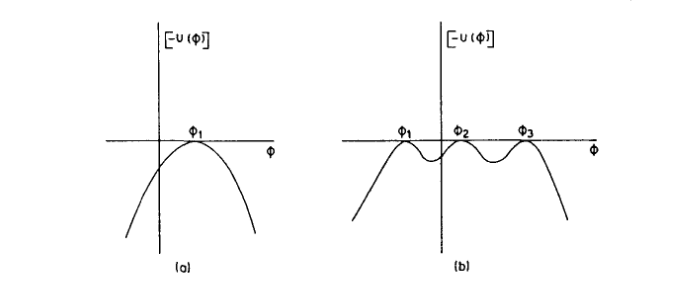
\includegraphics[height=6cm, width=14cm]{fig1}
\end{figure}

 Upon integrating (15) we get
 \begin{equation}%%%%%%%%%%16%%%%%%%%%%
 x - x_0 = \pm \int_{\phi(x_0)}^{\phi(x)}\frac{dz}{[2U(z)]^{1/2}}
 \end{equation}
 As an example let's consider the `kink' solution of the $\phi^4$ theory. The lagrangian density is of the form (8) with
 \begin{equation}%%%%%%%%%%17%%%%%%%%%%
 U(\phi) = \frac{1}{4}\lambda(\phi^2 - m^2/\lambda)^2
 \end{equation}
 where $\lambda$ and $m^2$ are positive constants. The equation of motion (9) becomes
 \begin{equation}%%%%%%%%%%18%%%%%%%%%%
 \ddot{\phi} - \phi'' = m^2 \phi - \lambda \phi^3
 \end{equation}
 
 The minimas of the potential are at $\phi = \pm m/\sqrt{\lambda}$. Using (16) we can solve for $\phi(x)$. The plus part is called kink and the negative is called antikink.
 
 \begin{equation}%%%%%%%%%%19%%%%%%%%%%
 \phi (x) = \pm (m/\sqrt{\lambda}) \textrm{tanh}[(m/\sqrt{2})(x - x_0)]
 \end{equation}
 $$ \epsilon (x) = \frac{1}{2}(\phi')^2  + U(\phi) = 2U(\phi) $$
 \begin{equation}%%%%%%%%%%20%%%%%%%%%%
 =(m^4/2\lambda)\textrm{ sech}^{4 }[(m/\sqrt{2})(x - x_0)]
 \end{equation}
  \begin{figure}[ht]
    \centering
    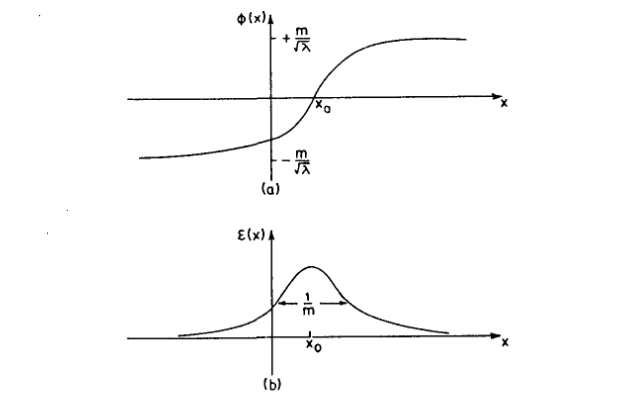
\includegraphics[height=9cm, width=13cm]{fig2}
\end{figure}
 
 \begin{equation}%%%%%%%%%%21%%%%%%%%%%
\phi_{kink}(x) = - \phi_{antikink}(x) = \phi_{antikink}(-x)
 \end{equation}
 
 The total kink energy, also called classical kinkmass $M_{cl}$ is given by
  \begin{equation}%%%%%%%%%%22%%%%%%%%%%
M_{cl} = \int_{-\infty}^{\infty} \epsilon (x) dx = \frac{2\sqrt{2}}{3}\frac{m^3}{\lambda}
 \end{equation}
 and is finite. The \textbf{kink and antikink} are therefore a legitimate \textbf{solitary wave}. However they are \textbf{not solitons}. This can be seen by taking two kink configuration and noticing that the first kink takes $\phi$ from $-m/\sqrt{\lambda}$ to $+m/\sqrt{\lambda}$ if this were followed by the second kink it will lead to $\phi = 2m/\sqrt{\lambda}$ which will lead to getting infinite energy.
 We can Lorentz transform the static solution in (19) to get the moving kink solution. 
 \begin{equation}%%%%%%%%%%23%%%%%%%%%%
 \phi_u (x,t) =  \frac{m}{\sqrt{\lambda}} \textrm{tanh}\bigg[\frac{m}{\sqrt{2}}\bigg(\frac{(x - x_0)-ut}{\sqrt{1-u^2}}\bigg)\bigg]
 \end{equation}
 We see that the spatial width of the moving kink is $\sqrt{1-u^2}/m$ as we would expect. Also putting all these into the enrgy function gives
   \begin{equation}%%%%%%%%%%24%%%%%%%%%%
\bm E[\phi_u]=\frac{M_{cl}}{\sqrt{1-u^2}}
 \end{equation}
 Another example is $U(\phi) = \frac{1}{2}\phi^2 (\phi^2 -1)^2$, which has three degenerate minimas. One would expect four types of static solutions here. Explicit static solutions in this case are:
 \begin{equation}
 \phi (x) = \pm (1+e^{\pm 2x})^{-1/2}.
 \end{equation}

 \section {Solitary waves in coupled scalar field in (1+1)d} 
 
Let us try to find static solutions to systems of coupled scalar fields in 1+1d. For $i=1,2,...,N$, consider the lagrangian density :
\begin{equation}%%%%%%%%%%26%%%%%%%%%%
\mathcal{L}(x,t) = \sum_{i=1}^{N}\frac{1}{2}[(\dot{\phi_i})^2 - (\phi'_i)^2 ] -U(\{\phi_i\})
\end{equation}
where $U(\{\phi_i\})$ is some function of all the $\phi_i$, having a minimal value of zero.
\begin{equation}%%%%%%%%%%27%%%%%%%%%%
 \square \phi_i  = -\frac{\partial U}{\partial \phi_i}; \quad \textrm{i=1,2,...,N.}
 \end{equation}
The static term must obey
\begin{equation}%%%%%%%%%%28%%%%%%%%%%
 \phi''_i = \frac{\partial U}{\partial \phi_i}
 \end{equation}
It's the same particle type intuition as before but now the particle is to move in N dimensions. Although it's similar to the previous case however there are two signifacnt differences when compared to a single-field case:\\
(i) There was no non-trivial solution when $U(\phi)$ had only 1 minima. Here however in the N-dimensional space particle can turn back towards it's starting point. Correspondingly a non-trivial solitary wave is possible.\\
(ii) Unlike the 1D case, there is no correspondingly simple way of integrating the coupled differential equations. We divide the task in two steps- First we find the 'orbit' analogue in the N-dimensional space and then we integrate along the orbit like a 1D problem. To determine the one-dimensional curve, we need to specify N-1 relations among the N coordinates $\phi_i(x)$. Finding all possible orbits from the potential is an extremely difficult problem.


  \begin{figure}[ht]
    \centering
    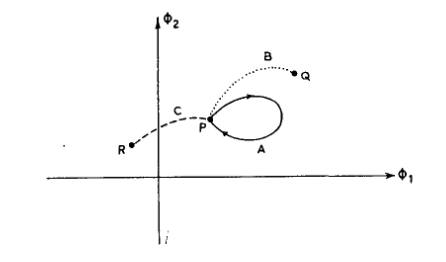
\includegraphics[height=6.27cm, width=11cm]{fig3}
\end{figure}
 

We illustrate this procedure with an example of two scalar field  coupled by $U(\phi_1,\phi_2)$. Let $U(\phi_1,\phi_2)$ have two degenerate minima at points P and Q in the $\{\phi_1,\phi_2\}$ as shown in the figure. The path from P to P is a type A path which is also called non-topological, the type B path from P to Q are called topological solutions and orbits of type C can not exist. Here for the 2D analogue we need only 1constraint. Let
\begin{equation}%%%%%%%%%29%%%%%%%%%%%%%
g(\phi_1,\phi_2) = 0
\end{equation}

be the equation of the orbit. We can then relate the orbit directly to the potential and eliminating x. We have then
$$\frac{dg}{dx} = 0 = \frac{\partial g}{\partial \phi_1} \phi '_1 + \frac{\partial g}{\partial \phi_2} \phi '_2. $$
which gives
\begin{equation}%%%%%%%%%30%%%%%%%%%%%%%
 \bigg(\frac{\partial g}{\partial \phi_1}\bigg)^2 (\phi '_1)^2 =  \bigg(\frac{\partial g}{\partial \phi_2}\bigg)^2 (\phi '_2)^2. 
 \end{equation}
Integrating (28), we get
\begin{equation}%%%%%%%%%31%%%%%%%%%%%%%
\frac{1}{2}(\phi'_i)^2 = \int \frac{\partial U(\phi_1,\phi_2)}{\partial \phi_i} d\phi_i  + A_i; \quad \textrm{i=1,2}
 \end{equation}
 Inserting (31) int (30) gives
 \begin{equation}%%%%%%%%%32%%%%%%%%%%%%%
 \bigg(\frac{\partial g}{\partial \phi_1}\bigg)^2 \bigg( \int \frac{\partial U(\phi_1,\phi_2)}{\partial \phi_1} d\phi_1  + A_1 \bigg) =  \bigg(\frac{\partial g}{\partial \phi_2}\bigg)^2 \bigg( \int \frac{\partial U(\phi_1,\phi_2)}{\partial \phi_2} d\phi_2  + A_2 \bigg)
 \end{equation}
The process of trying orbits is best illustrated by example. Consider a simple typical potential for coupled fields,
 \begin{equation}%%%%%%%%%33%%%%%%%%%%%%%
U(\phi_1,\phi_2) = \frac{1}{4}(\phi_1^2 - 1)^2  + \frac{1}{2}m^2(\phi_2)^2 + \frac{1}{4}\lambda(\phi_2)^2 + \frac{1}{2}d(\phi_1^2 - 1)^2 (\phi_2)^2
 \end{equation}
where $\lambda$, d and $m^2$ are all positive. The $U(\phi_1,\phi_2)$ has two absolute minima, at $\{-1,0\}$ and $\{1,0\}$. So orbits of type A and B may exist. For type B orbit let's try a path

 \begin{equation}%%%%%%%%%34%%%%%%%%%%%%%
g(\phi_1,\phi_2) = (\phi_2)^n + \alpha((\phi_1)^2 - 1 ) = 0
 \end{equation}
where $\alpha$ and n are the free parameters to be defined. Also it obeys that the two minimas lie on the path.
We can use equation (32) which gives us
 \begin{equation}%%%%%%%%%35%%%%%%%%%%%%%
(2\alpha\phi_1)^2 \bigg(\int_{-1}^{\phi_1} d\phi_1 (\phi_1^3 -\phi_1 + d\phi_2^2 \phi_1) \bigg) = (n\phi_2^{n-1})^2 \bigg(\int_{-1}^{\phi_2} d\phi_2 (m^2\phi_2 +\lambda \phi_2^3 + d\phi_2 (\phi_1^2 - 1)) \bigg)
 \end{equation}
where we used the boundary condition that $\phi'$ vanish vanish at the boundaries which gives $A_1$ and $A_2$ to be equal to zero. Now if we compare the coefficients we get two possible values of n. The solutions are: \\
(i) n=2, with \\
 \begin{equation}%%%%%%%%%36%%%%%%%%%%%%%
\alpha = \frac{(1-2m^2)}{d} \quad \textrm{and} \quad \lambda = \frac{d(d - 2m^2)}{1 - 2m^2}
 \end{equation}
 This simplifies  the equation of orbit(ellipse here) as
  \begin{equation}%%%%%%%%%37%%%%%%%%%%%%%
\phi_2^2 = [(1 - 2m^2)/d](1 - \phi_1^2)
 \end{equation}
 Inserting this into (28) gives us 
  \begin{equation}%%%%%%%%%38%%%%%%%%%%%%%
\phi_1'' = \phi_1^3 - \phi_1 + d\phi_2^2 \phi_1 = 2m^2 (\phi_1^3 - \phi_1)
 \end{equation}
 This can be easily integrated giving us
  \begin{equation}%%%%%%%%%39%%%%%%%%%%%%%
\phi_1 = \textrm{tanh}[m(x-x_0)]
 \end{equation}
 and
   \begin{equation}%%%%%%%%%40%%%%%%%%%%%%%
\phi_2 = \pm [(1 - 2m^2)/d]^{1/2} \textrm{sech}[m(x-x_0)]
 \end{equation}
(ii) n=1, with \\
 \begin{equation}%%%%%%%%%41%%%%%%%%%%%%%
\alpha^2 = \frac{(d - 3)}{d},  \quad \lambda = \frac{8}{3}d \quad \textrm{and} \quad m^2 = 2.
 \end{equation}
 This gives us a parabolic arc orbit:
  \begin{equation}%%%%%%%%%42%%%%%%%%%%%%%
\phi_2 = [(d - 3)/2d]^{1/2}(1 - \phi_1^2),
 \end{equation} 
  Inserting this into (28) gives us 
   \begin{equation}%%%%%%%%%43%%%%%%%%%%%%%
\phi_2'' = 2\phi_2 - d[2d/(d-3)]^{1/2}\phi_2^2+ \frac{8}{3}d\phi_2^3 
 \end{equation} 
 This has a standard form of an equation
    \begin{equation}%%%%%%%%%44%%%%%%%%%%%%%
\phi_2'' = a\phi_2 - \frac{3}{2}b\phi_2^2+ 2c\phi_2^3 
 \end{equation} 
 This is readily integrated to 
    \begin{equation}%%%%%%%%%45%%%%%%%%%%%%%
\phi_2(x) = \frac{2a}{(b^2 - 4ac)^{1/2}\textrm{cosh}(\sqrt{a}x)+ b}
 \end{equation} 
 and
 \begin{equation}%%%%%%%%%46%%%%%%%%%%%%%
\phi_1^2(x) = 1 - [2d/(d-3)]^{1/2} \phi_2,
 \end{equation} 
 Equation (39) and (45) both give us type B solution. They are shown in section (a) of the figure. While in section (b) of figure we have plotted the non-topological solutions which we will see below. For the same system we can try a type A orbit which begins and ends at (-1,0). The simplest choice is the ellipse given as
  \begin{equation}%%%%%%%%%47%%%%%%%%%%%%%
g(\phi_1,\phi_2) = (\phi_2)^2 + \beta(\phi_1 + 1 )(\phi_1 - \alpha ) = 0
 \end{equation}
 Again using (32) and comparing the coefficients we get the values 
   \begin{equation}%%%%%%%%%48%%%%%%%%%%%%%
\alpha = \frac{1+4m^2}{3}, \quad \beta = \frac{2-4m^2}{1+4m^2}, \quad d=\frac{3+12m^2}{4+4m^2}\quad\textrm{and}\quad \lambda = \frac{(5-4m^2)(1+4m^2)}{(8+8m^2)(1-2m^2)}.
 \end{equation} 
 Substituting this into (28) gives us an equation of the form (44) just $\phi_2$ replaced by $1+\phi_1$. Which gives us the solution of the form as
     \begin{equation}%%%%%%%%%49%%%%%%%%%%%%%
1+\phi_1(x) = \frac{2a}{(b^2 - 4ac)^{1/2}\textrm{cosh}(\sqrt{a}x)+ b}
 \end{equation} 

 
 
   \begin{figure}[ht]
    \centering
    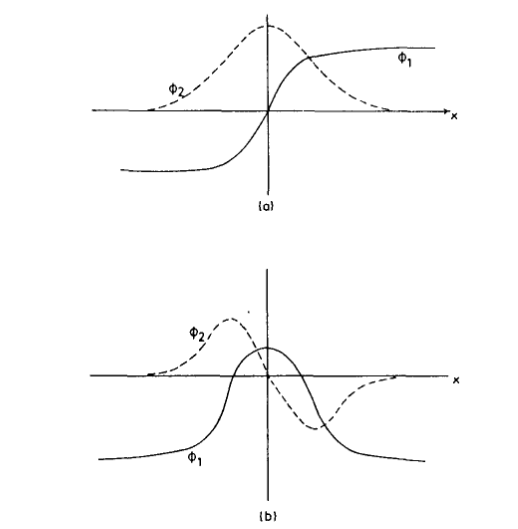
\includegraphics[height=9cm, width=12cm]{fig4}
   \end{figure}
  We observe that at the boundaries on both sides we get automatically the same limit so it is non-topological. Since it carries no non-zero topological index that could prevent it from dissipating into ripples, it may well be unstable.
 
 \section {Topological Indices}
    \begin{figure}[ht]
    \centering
    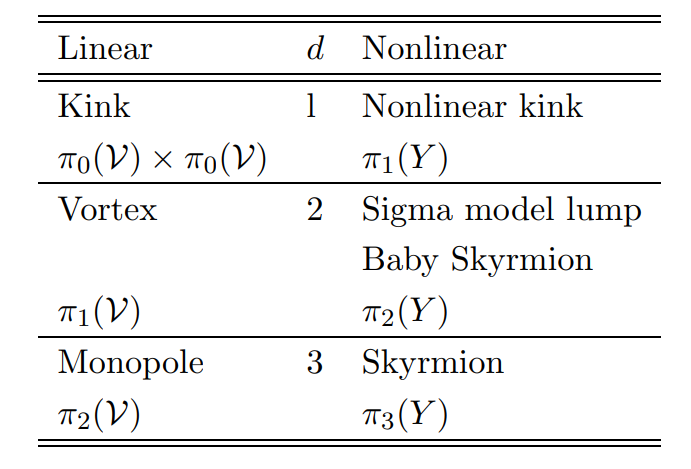
\includegraphics[height=7cm, width=12cm]{fig5}
   \end{figure}
 
 \section {Solitions of Sine-Gordon Equation}
 The solutions we have seen till now are solitary waves but not solitons. We will now consider a single scalar field in (1+1) dimensions, governed by the lagrangian density
 \begin{equation}%%%%%%%%%%50%%%%%%%%%%
\mathcal{L}(x,t) = \frac{1}{2}(\partial_{\mu}\phi)(\partial^{\mu}\phi) +(m^4/\lambda) \{\textrm{cos}[(\sqrt{\lambda}/m)\phi]-1\}
\end{equation}
 This system is used in the study of a wide range of  phenomena, including propagation of crystal dislocations, magnetic flux in Josephson lines and 2D models of elementary particles. We can expand the lagrangian density in powers of the coupling constant as
  \begin{equation}%%%%%%%%%%51%%%%%%%%%%
\mathcal{L}(x,t) = \frac{1}{2}(\partial_{\mu}\phi)(\partial^{\mu}\phi) -\frac{1}{2}m^2 \phi^2 + \frac{\lambda}{4!}\phi^4 + ...
\end{equation}
 This gives rise to an equation of motion similar to the Klien-Gordon equation called the Sine-Gordon equation:
   \begin{equation}%%%%%%%%%%52%%%%%%%%%%
\square \phi + (m^3/\lambda)\textrm{sin}[(\sqrt{\lambda}/m)\phi]
\end{equation}
 Returning to the equation we do a change in variables as follows:
    \begin{equation}%%%%%%%%%%53%%%%%%%%%%
\bar{x}=mx, \quad \bar{t}= mt \quad\textrm{and} \quad\bar{\phi}=(\sqrt{\lambda}/m)\phi
\end{equation}
The lagrangian density becomes
  \begin{equation}%%%%%%%%%%54%%%%%%%%%%
\mathcal{\bar{L}}(x,t) = (m^4/\lambda)\bigg[\frac{1}{2}(\partial_{\mu}\phi)(\partial^{\mu}\phi) +(\textrm{cos}\phi -1
)\bigg]
\end{equation}

 \begin{equation}%%%%%%%%%%55%%%%%%%%%%
\frac{\partial^2\phi}{\partial t^2} - \frac{\partial^2\phi}{\partial x^2} +\textrm{sin}\phi(x,t)=0
\end{equation}
 \begin{equation}%%%%%%%%%%56%%%%%%%%%%
\bm  E[\phi] =\frac{m^3}{\lambda} \int_{\infty}^{-\infty} dx \bigg[ \frac{1}{2}\bigg(\frac{\partial\phi}{\partial t}\bigg)^2 +\frac{1}{2}\bigg(\frac{\partial\phi}{\partial x}\bigg)^2 +(1 -\textrm{cos}\phi
) \bigg]
 \end{equation}

Note that the enrgy functional vanishes when $\phi=2N\pi\quad (N=...,-2,-1,0,1,2,...)$
We observe that the lagrangian and the field equations enjoy discrete symmetries-
$$\phi(x,t) \to -\phi(x,t)$$
 \begin{equation}%%%%%%%%%%57%%%%%%%%%%
\phi(x,t) \to \phi(x,t)+2N\pi;\quad N=...,-2,-1,0,1,2,...
\end{equation}
Using (16) we can solve the equation as
 \begin{equation}%%%%%%%%%%58%%%%%%%%%%
 x - x_0 = \pm \int_{\phi(x_0)}^{\phi(x)}\frac{dz}{[2U(z)]^{1/2}} = \pm \int_{\phi(x_0)}^{\phi(x)}\frac{dz}{2\textrm{sin}(z/2)}
 \end{equation}
  \begin{figure}[ht]
    \centering
    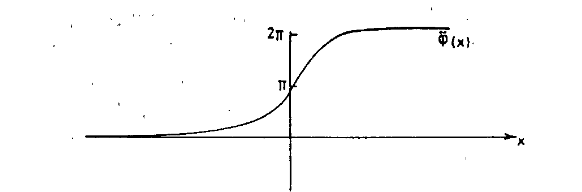
\includegraphics[height=7cm, width=12cm]{fig6}
   \end{figure}
This can be integrated and which gives
 \begin{equation}%%%%%%%%%%59%%%%%%%%%%
\phi(x)=4\textrm{tan}^{-1}[\textrm{exp}(x-x_0)] \equiv \phi_{sol}(x-x_0)
 \end{equation}
 or
  \begin{equation}%%%%%%%%%%60%%%%%%%%%%
\phi(x)=-4 \textrm{tan}^{-1}[\textrm{exp}(x-x_0)] \equiv \phi_{antisol}(x-x_0)
 \end{equation}
 Here we note that suppose we have two kink solutions while the first kink takes the analogous particle from 0 to $2\pi$ the second kink takes it from $2\pi$ to $4\pi$. But we know that energy vanishes at $2N\pi$, so the adding the localised solution doesnot blow up the energy. It can be calculated and seen that adding the localised solutions at t$\to -\infty$ and evolving them and then taking the limit at at t$\to +\infty$ remains the same. Hence these solitary waves satisfy the condition to be called a \textbf{soliton}.\\
 The general solution doing lorentz transform and then evolving the soliton-antisoliton and the soliton-soliton pair is given as:
 \begin{equation}%%%%%%%%%%61%%%%%%%%%%
 \phi_{SA}(x,t) = 4\textrm{tan}^{-1}\bigg(\frac{\textrm{sinh}(ut/\sqrt{1-u^2})}{u\*\ \textrm{cosh}(x/\sqrt{1-u^2})}\bigg)
 \end{equation}
 and
  \begin{equation}%%%%%%%%%%62%%%%%%%%%%
 \phi_{SS}(x,t) = 4\textrm{tan}^{-1}\bigg(\frac{u\*\ \textrm{sinh}(x/\sqrt{1-u^2})}{\textrm{cosh}(ut/\sqrt{1-u^2})}\bigg)
 \end{equation}
 From the equations one can see that soliton and antisoliton attract each other and soliton and soliton repel each other.


  \section {References}
1. Solitons and Instantons by R. Rajaraman.\\
2. Topological Solitons by Manton and Sutcliffe.
\end{document}